\section{TASK 2, Setting up the neural network for Euler's method}

\begin{frame}
	\frametitle{Euler's Method}
	\paragraph{Formula:}\vspace{-1mm}
	\quad\quad $y_{n+1} = y_n + h \cdot \dot{y}_n$
	\vspace{1mm}
	
	\paragraph{Properties:}\vspace{-2mm}
	\begin{itemize}
		\item Black-Box-Approach
		\item Explicit numerical integration
		\begin{itemize}
			\item[$\Rightarrow$] No RNN required
		\end{itemize}
	\end{itemize}
	
	\paragraph{Architecture}\vspace{2mm}
	\begin{figure}[H]
		\centering
		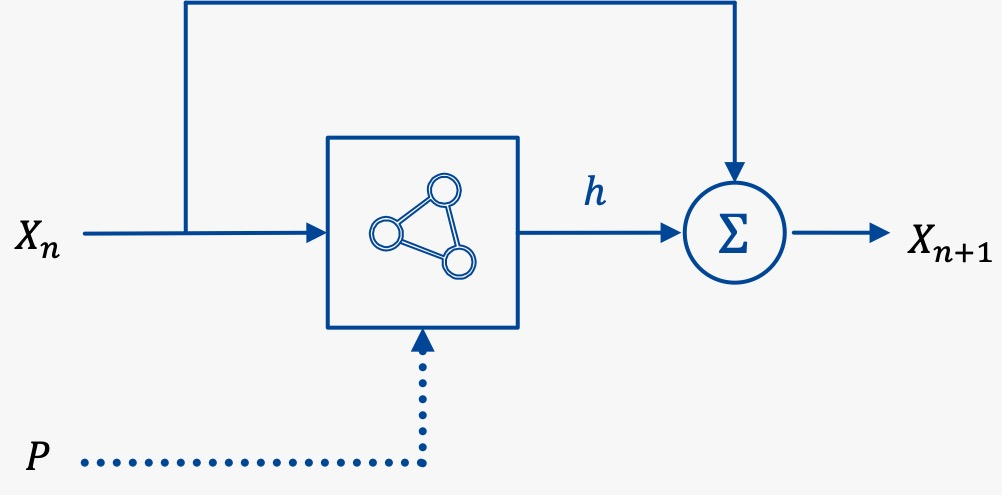
\includegraphics[width=.5\linewidth]{figures/euler/net_architecture}
	\end{figure}
\end{frame}

\begin{frame}
	\frametitle{Network configuration}
	\centering
	\begin{tabular} { c | c | c | c}
						& Linear System & Andronov-Hopf & R\"ossler attractor	\\
		\hline
		Input			& 2 		& 2			& 3			\\
		\hline
		Parameters		& 0 		& 1			& 1			\\
		\hline
		Hidden layers	& 2			& 3			& 3			\\
		\hline
		Neurons / layer	& 20		& 100		& 200		\\
		\hline
		Output			& 2			& 2			& 3			\\
		\hline
		Loss function	& MSE		& MSE		& MSE		\\
		\hline
		Optimization	& SGD		& Adam		& Adam		\\
	\end{tabular}
\end{frame}
